\documentclass[letterpaper]{article}
\usepackage[utf8]{inputenc}
\usepackage[spanish]{babel}
\usepackage{amssymb, amsmath}
\usepackage{graphicx}
\usepackage{lipsum}
\usepackage{dsfont}
\usepackage[margin=1.5cm,
vmargin={1.5cm,1.3cm},
includefoot]{geometry}
\usepackage{setspace}
\usepackage{subcaption}
\usepackage{tocloft}
\usepackage{upgreek}
\usepackage{amsthm}
\usepackage{graphicx}
\usepackage{paralist}
\usepackage{fancyhdr}
\usepackage{lmodern}
\usepackage{tcolorbox}
\usepackage{color}
\usepackage{tikz}
\usepackage{wasysym}
\usepackage{textgreek, marvosym}
\tcbuselibrary{skins,breakable}
\pagestyle{fancy}

\renewcommand{\headrulewidth}{0.4pt}
\renewcommand{\footrulewidth}{0.4pt}

\renewcommand{\d}{\partial}

\providecommand{\abs}[1]{\left|#1\right|}
\providecommand{\norm}[1]{\left|\left|#1\right|\right|}														  
\newcommand{\V}{\mathds{V}}

\newcommand{\W}{\mathds{W}}

\newcommand{\F}{\mathds{F}}

\newcommand{\tq}{ \quad \cdot  \backepsilon \cdot \quad }

\newcommand{\ld}{\lim\limits_{x \to 0^{+}}}

\newcommand{\li}{\lim\limits_{x \to 0^{-}}}

\newcommand{\la}{\lim\limits_{x \to a}}

\newcommand{\R}{\mathds{R}}

\newcommand{\Po}{\mathds{P}_2(\mathds{R})}

\renewcommand{\*}{\cdot}

\newcommand{\Iden}{\begin{pmatrix}
		1 & 0 & 0\\
		0 & 1 & 0\\
		0 & 0 & 1 
\end{pmatrix}}
\newcommand{\T}{\begin{pmatrix}
		1 & 3 & 9 \\
		1 & 3 & 4 \\
		0 & 0 & 2 
\end{pmatrix} }

\makeatletter
\renewcommand*\env@matrix[1][\arraystretch]{%
	\edef\arraystretch{#1}%
	\hskip -\arraycolsep
	\let\@ifnextchar\new@ifnextchar
	\array{*\c@MaxMatrixCols c}}
\makeatother

\newtheorem{theorem}{Teorema}[section]
\theoremstyle{definition}
\newtheorem{definition}{Definición}


\begin{document}
	
	\setlength{\unitlength}{1cm}
	\thispagestyle{empty}
	\begin{picture}(19,3)
	\put(-0.5,1.2){
\includegraphics[scale=.20]{img/unam1.png}}
	\put(16,1){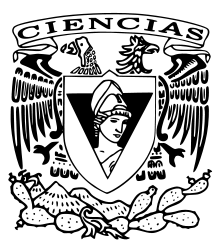
\includegraphics[scale=.29]{img/fciencias1.png}}
	\end{picture}
	
	\begin{center}
		\vspace{-114pt}
		\textbf{\large Matemáticas para las Ciencias II}\\
		\textbf{ Semestre 2020-2}\\
		Prof. Pedro Porras Flores\\
		Ayud. Irving Hernández Rosas \\
		\textbf{Proyecto III}\\[0.2cm]
		Kevin Ariel Merino Peña\footnote{Número de cuenta 317031326}\\ [0.2cm]
	\end{center}
	\vspace{-10pt}
	\rule{19cm}{0.3mm}
	
\noindent Realice los siguientes ejercicios, escribiendo el procedimiento claramente. Y recuerden que estos proyectos se entregan de manera individual en la plataforma de google classroom.\\




% -----------------------------------------------------
% Problema uno
% -----------------------------------------------------

\noindent1.  Calcule la matriz de la derivadas parciales de: 

\begin{definition}
	Ses $ U $ un conjunto abierto en $ \R^n $ y sea $ f:U\subset \R^n \to \R^m $. Se dice que $ f $ es diferenciable en $ \vec{x_0} \in U$  si todas las derivadas parciales existen y además si el siguiente límite existe: 
	\[ \lim\limits_{\vec{x} \to \vec{x_0} } \dfrac{\norm{f(\vec{x}) - f(\vec{x_0}) - T(\vec{x} - \vec{x_0})} }{\norm{\vec{x} - \vec{x_0}}} =0 \]
	Donde $ T= Df(\vec{x_0}) \in M_{mxn} $ cuyos elementos son $ \dfrac{\partial f_i}{\partial x_j} $ con $ 1 \leq i \leq m $ y $ 1 \leq j \leq n $. Esto es
	\begin{align*}
		Df(\vec{x_0}) &= \begin{pmatrix}[2.5]
		\dfrac{\partial f_1}{\d x_1 } & \dfrac{\d f_1}{\d x_2} & \dots & \dfrac{\d f_1}{\d x_n}\\
		\dfrac{\partial f_2}{\d x_1 } & \dfrac{\d f_2}{\d x_2} & \dots & \dfrac{\d f_2}{\d x_n}\\
		\vdots & & \ddots & \\
		\dfrac{\partial f_m}{\d x_1 } & \dfrac{\d f_m}{\d x_2} & \dots & \dfrac{\d f_m}{\d x_n}\\
		\end{pmatrix}
	\end{align*}
	Es llamada matriz de las derivadas parciales o Matriz Jacobiana
\end{definition}

\noindent a) $f: \mathbb{R}^2  \longrightarrow \mathbb{R}^2$, tal que $f(x,y) = (e^x,\sin(xy))$
\begin{align*}
	Df(\vec{x_0}) &= \begin{pmatrix}[2.5]
	\dfrac{\d e^x}{\d x} & \dfrac{\d e^x}{\d y}\\
	\dfrac{\d \sin(xy)}{\d x} & \dfrac{\d \sin(xy)}{\d y}\\
	\end{pmatrix} && \text{Por definición de la matriz Jacobiana}\\
	Df(\vec{x_0}) &= \begin{pmatrix}[2.5]
	e^x & \dfrac{\d e^x}{\d y}\\
	\dfrac{\d \sin(xy)}{\d x} & \dfrac{\d \sin(xy)}{\d y}\\
	\end{pmatrix} && \text{La derivada de $ e^x $ es la función misma (cálculo I)}\\
	Df(\vec{x_0}) &= \begin{pmatrix}[2]
	e^x & 0\\
	\dfrac{\d \sin(xy)}{\d x} & \dfrac{\d \sin(xy)}{\d y}\\
	\end{pmatrix} && \text{Puesto que $ x $ figura como constante}\\
	Df(\vec{x_0}) &= \begin{pmatrix}[2]
	e^x & 0\\
	y\dfrac{\d \sin(xy)}{\d x} & x\dfrac{\d \sin(xy)}{\d y}\\
	\end{pmatrix} && \text{Por regla de la cadena}\\
	Df(\vec{x_0}) &= \begin{pmatrix}[1.5]
	e^x & 0\\
	y\cos(xy) &x\cos(xy)\\
	\end{pmatrix} && \text{Efectuando las derivadas parciales}\\
\end{align*}


\noindent b) $f: \mathbb{R}^2  \longrightarrow \mathbb{R}^3$, tal que $f(x,y) = (xe^y + \cos(y), x, x + e^y)$

\begin{align*}
	Df(\vec{x_0}) &= \begin{pmatrix}[2.5]
	\dfrac{\d}{\d x} (xe^y + \cos(y)) & \dfrac{\d}{\d y} (xe^y + \cos(y))\\
	\dfrac{\d}{\d x} x & \dfrac{\d}{\d y} x\\
	\dfrac{\d}{\d x} (x + e^y) & \dfrac{\d}{\d y}( x + e^y)\\
	\end{pmatrix} &&\text{Por definición de matriz de derivadas parciales}\\
	Df(\vec{x_0}) &= \begin{pmatrix}[2.5]
	  e^y\dfrac{\d}{\d x} x + \dfrac{\d}{\d x}\cos(y) & x\dfrac{\d}{\d y} e^y + \dfrac{\d}{\d y}\cos(y)\\
	\dfrac{\d}{\d x} x & \dfrac{\d}{\d y} x\\
	\dfrac{\d}{\d x} x + \dfrac{\d}{\d x}e^y & \dfrac{\d}{\d y} x + \dfrac{\d}{\d y}e^y\\
	\end{pmatrix} &&\text{Empleamos que la derivada es lineal, abre sumas y saca escalares}\\
	Df(\vec{x_0}) &= \begin{pmatrix}[1.5]
	e^y & x e^y - \sin(y)\\
	1 & 0\\
	1 & e^y\\
	\end{pmatrix} &&\text{Operando las derivadas}
\end{align*}

\noindent c) $f: \mathbb{R}^3  \longrightarrow \mathbb{R}^2$, tal que $f(x,y,z) = (x + e^z + y, xy^2)$
\begin{align*}
	Df(\vec{x_0}) &= \begin{pmatrix}[2.5]
	\dfrac{\d}{\d x} (x + e^z + y) & \dfrac{\d}{\d y} (x + e^z + y) & \dfrac{\d}{\d z} (x + e^z + y) \\
	\dfrac{\d}{\d x} (xy^2) & \dfrac{\d}{\d y}( xy^2) & \dfrac{\d}{\d z} (xy^2) \\
	\end{pmatrix} && \text{Por definición de la matriz de derivadas parciales}\\
	Df(\vec{x_0}) &= \begin{pmatrix}[2.5]
	\dfrac{\d}{\d x} x + \dfrac{\d}{\d x} e^z + \dfrac{\d}{\d x} y & \dfrac{\d}{\d y} x + \dfrac{\d}{\d y} e^z +\dfrac{\d}{\d y} y & \dfrac{\d}{\d z} x + \dfrac{\d}{\d z} e^z + \dfrac{\d}{\d z}y \\
	y^2\dfrac{\d}{\d x} x & x\dfrac{\d}{\d y}y^2 & \dfrac{\d}{\d z} (xy^2) \\
	\end{pmatrix} && \text{Usamos que la derivada es un operador lineal}\\
	Df(\vec{x_0}) &= \begin{pmatrix}[1.5]
	1& 1 & e^z \\
	y^2 & 2xy & 0 
	\end{pmatrix} && \text{Efectuando las derivadas parciales}
\end{align*}

\noindent d) $f: \mathbb{R}^3  \longrightarrow \mathbb{R}^3$, tal que $f(x,y,z) = (xye^{xy}, x\sin(y), 5xy^2)$
\begin{align*}
	Df(\vec{x_0}) &= \begin{pmatrix}[2.5]
	\dfrac{\d }{\d x} xye^{xy}  & \dfrac{\d }{\d y} xye^{xy}  & \dfrac{\d }{\d z} xye^{xy} \\
	\dfrac{\d }{\d x} x\sin(y) & \dfrac{\d }{\d y} x\sin(y) & \dfrac{\d }{\d z} x\sin(y) \\
	\dfrac{\d }{\d x}  5xy^2 & \dfrac{\d }{\d y}  5xy^2 & \dfrac{\d }{\d z}  5xy^2 
	\end{pmatrix} && \text{Definición de matriz de derivadas parciales}\\
	Df(\vec{x_0}) &= \begin{pmatrix}[2.5]
	y\dfrac{\d }{\d x} e^{xy}x  & x\dfrac{\d }{\d y} ye^{xy}  & \dfrac{\d }{\d z} xye^{xy} \\
	\sin(y)\dfrac{\d }{\d x} x & x\dfrac{\d }{\d y} \sin(y) & \dfrac{\d }{\d z} x\sin(y) \\
	5y^2\dfrac{\d }{\d x}  x & 5x\dfrac{\d }{\d y}  y^2 & \dfrac{\d }{\d z}  5xy^2 
	\end{pmatrix} && \text{Empleando que la derivada es operador lineal}
\end{align*}
\begin{align*}
	Df(\vec{x_0}) &= \begin{pmatrix}[2.5]
	y(e^{yx} + xye^{xy})  & x(e^{xy} + xye^{xy})  & 0 \\
	\sin(y) & x\cos(y) & 0 \\
	5y^2 & 10xy & 0 
	\end{pmatrix} && \text{Operando las dervidas parciales}
\end{align*}

\noindent 2.  Sea $f(x,y) = xe^{y^2} - ye^{x^2}$\\


\noindent a) Encuentre el plano tangente a la gráfica de $f$ en $(1, 2)$\\

\noindent b) ¿Qué punto sobre la superficie $z = x^2 -y^2$, tiene un plano tangente paralelo al plano tangente encontrado en la primer parte?\\


\noindent 3.  Calcule el gradiente de las siguientes funciones:\\


\noindent a) $f(x,y,z) = x e^{-(x^2 +y^2 +z^2)}$\\

\noindent b) $f(x,y,z) = \dfrac{xyz}{x^2 +y^2 +z^2}$\\

\noindent c) $f(x,y,z) = z^2e^x\cos(y)$\\



\noindent 4. Haga un bosquejo de las curvas que son las imágenes de las siguientes trayectorias:\\


\noindent a) $\vec{\gamma}(t) = (\sin(t), 4\cos(t))$, donde $0 \leq t \leq 2\pi$\\

\noindent b) $\vec{\gamma}(t) = (2\sin(t), 4\cos(t))$, donde $0 \leq t \leq 2\pi$\\

\noindent c) $\vec{\gamma}(t) = (t\sin(t), t\cos(t), t)$, donde $ -4\pi \leq t \leq 4\pi$\\


\noindent 5. El vector de posición para una partícula que se mueve sobre una hélice es: $$\vec{\gamma}(t) = (\sin(t), \cos(t), t^2)$$


\noindent a) Encuentre la rapidez de la partícula en el tiempo  $t_0 = 4\pi$\\

\noindent b) ¿Es $\vec{\gamma}$ es ortogonal a  $\vec{\gamma'}$\\

\noindent c) Encuentre la recta tangente a $\vec{\gamma}$ $t_0 = 4\pi$\\

\noindent d) ¿Dónde se intersecará esta línea con el plano $xy$?\\





\end{document}
